\documentclass[a4paper, 12pt, titlepage]{article}

% Including needed packages
\usepackage[margin=2cm]{geometry}
\usepackage{amsmath}
\usepackage{amssymb}
\usepackage{amsthm}
\usepackage{graphicx}
\usepackage{subfig}
\usepackage{float}


\newcommand{\norm}[1]{\lVert#1\rVert}

\title
{{\em Machine learning 2}\\
Exercise sheet 5}
\author{FLEISCHMANN Kay, Matrnr: 352247\\
	ROHRMANN Till, Matrnr: 343756}
\date{\today}

\begin{document}

\maketitle

\section{One-class-SVM: Theory}
\subsection*{(a) Derive the dual program for the one-class SVM.}
\subsubsection*{Primal form}

The primal form of the one-class SVM has the following form:

\begin{equation*}
	\min_{\boldsymbol{\mu},r,\boldsymbol{\xi}} r^2 + C\sum_{i=1}^N \xi_i
\end{equation*}
such that
\begin{eqnarray*}
	\norm{\phi(x_i)-\boldsymbol{\mu}}^2 &\le& r^2 + \xi_i\\
	\xi_i &\ge& 0
\end{eqnarray*}

for $i=1,\ldots,n$. Using Lagrange multipliers gives us the unconstrained form:

\begin{eqnarray*}
	\min_{\boldsymbol{\mu},r,\boldsymbol{\xi}}\max_{\boldsymbol{\alpha},\boldsymbol{\beta} \ge 0} \underbrace{ \left\{ r^2 + C\sum_{i=1}^N \xi_i + \sum_{i=1}^N \alpha_i \left( \norm{\phi(x_i)-\boldsymbol{\mu}}^2 -r^2 - \xi_i\right) -\sum_{i=1}^N \beta_i \xi_i\right\}}_{L(\boldsymbol{\mu},r,\boldsymbol{\xi},\boldsymbol{\alpha},\boldsymbol{\beta})} 
\end{eqnarray*}

The dual optimization problem is now given by 
\begin{eqnarray*}
	\max_{\boldsymbol{\alpha},\boldsymbol{\beta} \ge 0} g(\boldsymbol{\alpha},\boldsymbol{\beta})
\end{eqnarray*}

with $g$ being defined by

\begin{eqnarray}
	g(\boldsymbol{\alpha},\boldsymbol{\beta}) &=& \min_{\boldsymbol{\mu},r,\boldsymbol{\xi}} L(\boldsymbol{\mu},r,\boldsymbol{\xi},\boldsymbol{\alpha},\boldsymbol{\beta}) \label{eq:g}
\end{eqnarray}

To compute the minimum of $L$ w.r.t. $\boldsymbol{\mu}, r$ and $\boldsymbol{\xi}$ we take the partial derivative and set it afterwards to zero.

\begin{eqnarray}
	\nabla_{\boldsymbol{\mu}} L &=& \nabla_{\boldsymbol{\mu}} \left( \sum_{i=1}^N \alpha_i \left( \phi(x_i) - \boldsymbol{\mu} \right)^T \left( \phi(x_i) - \boldsymbol{\mu} \right) \right) \nonumber \\
	&=& \sum_{i=1}^N \alpha_i\left( 2 \boldsymbol{\mu} - 2 \phi(x_i) \right) \label{eq:mu}\\
	\frac{\partial L}{\partial r} &=& 2r -2\sum_{i=1}^N \alpha_i r \label{eq:r}\\
	\frac{\partial L}{\partial \xi_j} &=& C - \alpha_j - \beta_j \label{eq:xi}
\end{eqnarray}

Setting equations \eqref{eq:mu},\eqref{eq:r} and \eqref{eq:xi} to $0$ we obtain

\begin{eqnarray}
	\boldsymbol{\mu} \sum_{i=1}^N \alpha_i &=& \sum_{i=1}^N \alpha_i \phi(x_i) \label{eq:mualpha}\\
	(1-\sum_{i=1}^N \alpha_i)r &=& 0 \label{eq:alpha}\\
	C &=& \alpha_i + \beta_i \label{eq:C}
\end{eqnarray}

Assuming that we have at least 2 distinct data points, we know that $r>0$ holds. Thus equation \eqref{eq:alpha} gives us
\begin{eqnarray}
	\sum_{i=1}^N \alpha_i &=& 1 \label{eq:alpha1}
\end{eqnarray}

and thus equation \eqref{eq:mualpha} can be expressed by
\begin{eqnarray}
	\boldsymbol{\mu} &=& \sum_{i=1}^N\alpha_i \phi(x_i) \label{eq:mu2}
\end{eqnarray}

This equation says that one can express the optimal solution for $\boldsymbol{\mu}$ as a linear combination of the data points in feature space.
Plugging equations \eqref{eq:C} and \eqref{eq:mu2} into equation \eqref{eq:g} gives us
\begin{eqnarray}
	g(\boldsymbol{\alpha},\boldsymbol{\beta}) &=& r^2 + \sum_{i=1}^N (\alpha_i+\beta_i) \xi_i + \sum_{i=1}^N \alpha_i \left( \norm{\phi(x_i)-\sum_{i=1}^N\alpha_i \phi(x_i)}^2 -r^2 - \xi_i\right) -\sum_{i=1}^N \beta_i \xi_i \nonumber\\
	&=& r^2 -r^2\sum_{i=1}^N\alpha_i + \sum_{i=1}^N\alpha_i \left( \phi(x_i)-\sum_{j=1}^N\alpha_j \phi(x_j) \right)^T \left(\phi(x_i)-\sum_{j=1}^N\alpha_j \phi(x_j)\right) \nonumber
\end{eqnarray}
Using equation \eqref{eq:alpha1} gives us
\begin{eqnarray*}
	g(\boldsymbol{\alpha}) &=& \sum_{i=1}^N \alpha_i \phi(x_i)^T\phi(x_i) - \sum_{i,j=1}^N\alpha_i\alpha_j \phi(x_i)^T\phi(x_j)
\end{eqnarray*}
with the additional constraints
\begin{eqnarray*}
	\sum_{i=1}^N\alpha_i &=&1\\
	C = \alpha_i + \beta_i &\Rightarrow& 0 \le \alpha_i \le C
\end{eqnarray*}

Assuming we have a kernel function $k$ expressing the inner product $\phi(x)^T\phi(y)=k(x,y)$ we finally end up at the final formulation:

\begin{eqnarray}
	\max_{\boldsymbol{\alpha}} \left\{ \sum_{i=1}^N\alpha_ik(x_i,x_i) - \sum_{i,j=1}^N\alpha_i\alpha_jk(x_i,x_j) \right\} \label{eq:final}
\end{eqnarray}
subject to
\begin{eqnarray*}
	\sum_{i=1}^N\alpha_i &=&1\\
	0 \le \alpha_i &\le& C \text{ with } i=1,\ldots,n
\end{eqnarray*}

\subsection*{(b) Show that the dual problem is a linearly constrained quadratic problem.}

Setting $\left(\boldsymbol{b}\right)_i = k(x_i,x_i)$ and $\left(A\right)_{i,j} = -k(x_i,x_j)$ we can reformulate equation \eqref{eq:final} in its matrix/vector notation

\begin{eqnarray*}
	\eqref{eq:final} &=& \max_{\boldsymbol{\alpha}} \boldsymbol{\alpha}^TA\boldsymbol{\alpha} + \boldsymbol{b}^T\boldsymbol{\alpha}
\end{eqnarray*}

Furthermore by setting $v=1$, $\boldsymbol{u} = \begin{bmatrix}1\\ \vdots \\ 1\end{bmatrix}, l_i = 0$ and $m_i=C$ for $i=1,\ldots,n$ we can rewrite the constraints:

\begin{eqnarray*}
	\sum_{i=1}^N \alpha_i = 1 &\Leftrightarrow& \boldsymbol{u}^T\boldsymbol{\alpha} = v\\
	0 \le \alpha_i \le C &\Leftrightarrow& l_i \le \alpha_i \le m_i
\end{eqnarray*}

\section{Implementation} see attached matlab implementation. \newline
$pr\_loqo2$ is running into small value (close to zero) issues. Tested with 64Bit/Win7/(Matlab 2012 b/2013a). quadprog() worked instead.

\section{Result of the One-class SVM vs. hackers}

With the help of the slack-variables $\xi_i$ the One-class-SVM try to fit best on the normal data in order to find the anormal hacker activities. Using an appropriate value of $C$ is important to distinguish hacker activities from normal ones.
The following plot shows the number of hacker activities found if $C$ ist changed, starting with $C=1$ and halved in each step.

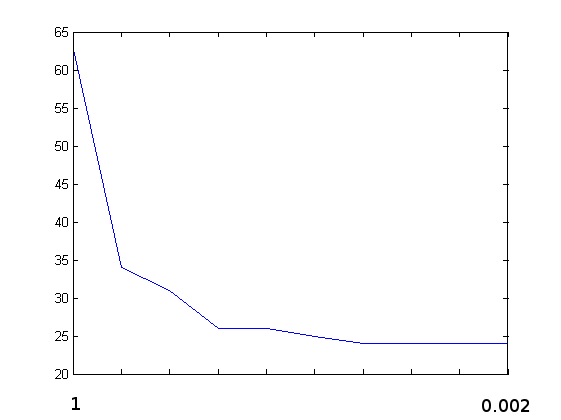
\includegraphics[width=0.7\textwidth]{images/plot_found_hackers.png}

Maybe an appropriate value for may $C=0.002$. This value is applied to test data to find hacker activities on event-logs.

\subsection*{Hacker atttacks found}

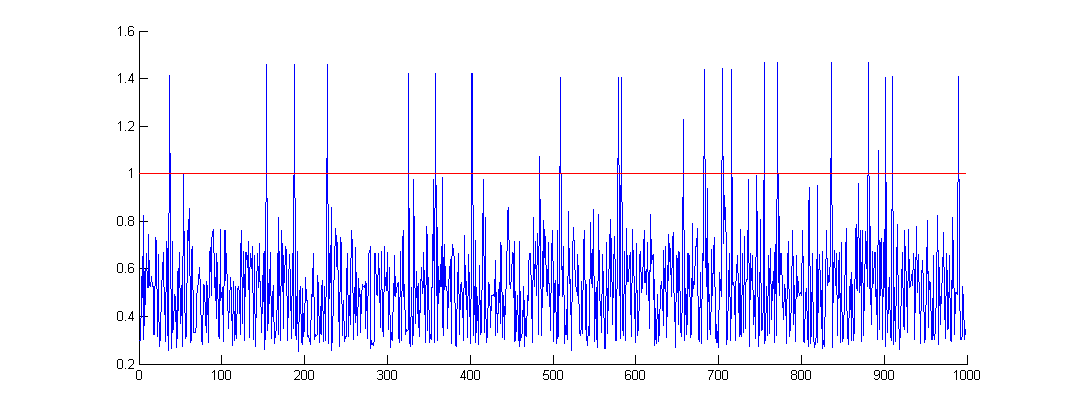
\includegraphics[width=\textwidth]{images/plot_testdata.png}

\subsection*{Explicit position of hacker attacks}
    37
   154
   188
   228
   326
   358
   402
   403
   484
   509
   579
   583
   658
   683
   705
   716
   755
   771
   836
   881
   893
   902
   910
   990


\end{document}
